\section {Texto Simples}
As seções com texto simples estarão dispostas desta maneira. Além das seções
também será possível adionar até quatro níveis.

\subsection{Segundo nível}
Também temos dois tipos de citação:

Citação normal, no final da frase \cite{Flores2016,Soares2013}. Ou podemos
também utilizar a citação dentro do texto como por exemplo:
\citeonline{Flores2016} fez algumas coisas legais e mais algun texto explicando
alguma coisa que \citeonline{Soares2013}.



\subsubsection{Terceiro nível}
Podemos fazer uso de ítens:
\begin{itemize}
  \item Algum texto 1
  \item Algum texto 2
  \item Algum texto 3
\end{itemize}
depois o texto continua da mesma maneira.

\subparagraph{Quarto nível}
Algum texto

\section {Equações}
As equações são numeradas automaticamente. Também podemos utilizar a referência
cruzada para as equações

\subsection{Equações simples}
A \autoref{eq:nrtl} é o modelo de coeficiente de atividade NRTL
\begin{equation}\label{eq:nrtl}
\ln \gamma_i = \frac{\displaystyle\sum_j x_j \tau_{ji}
G_{ij}}{\displaystyle\sum_k x_k G_{ki}} + \displaystyle\sum_j \frac{x_j G_{ij}}{\displaystyle\sum_k x_k G_{kj}}\left(
\tau_{ij} - \frac{\displaystyle\sum_m x_m \tau_{mj} G_{mj}}{\displaystyle\sum_k x_k G{kj}} \right)
\end{equation}

Podemos também escrever a \autoref{eq:nrtl} de forma mais comprimida
\begin{equation}\tag{\ref{eq:nrtl}}
\ln \gamma_i = \frac{\sum_j x_j \tau_{ji} 
G_{ij}}{\sum_k x_k G_{ki}} + \sum_j \frac{x_j G_{ij}}{\sum_k x_k G_{kj}}\left(
\tau_{ij} - \frac{\sum_m x_m \tau_{mj} G_{mj}}{\sum_k x_k G{kj}} \right)
\end{equation}
onde
\begin{align}
\tau_{ji} &= \frac{g_{ij} - g_{ii}}{RT}\\
G_{ji} &= \rho_{ji} \exp{ \left(-\alpha_{ji} \tau_{ji}\right)} \label{eq:nrtlg}
\end{align}

Também podemos utilizar subequações
\begin{subequations}
\begin{align}
\tau_{ji} &= \frac{g_{ij} - g_{ii}}{RT}\\
G_{ji} &= \rho_{ji} \exp{ \left(-\alpha_{ji} \tau_{ji}\right)} \label{eq:nrtlg}
\end{align}
\end{subequations}


\subsection{Equações longas}
Também podemos escrever equações muito longas, como a \autoref{eq:nrtl2} 
\begin{equation}\label{eq:nrtl2}
\begin{aligned} 
\ln \gamma_i = &q \left(1- \ln \sum_j x_j G_{ji} - \sum_j \frac{x_j
G_{ij}}{\sum_k x_k G_{kj}} \right) \\
&+ p\left[ \frac{\sum_j x_j \tau_{ji}
G_{ij}}{\sum_k x_k G_{ki}} + \sum_j \frac{x_j G_{ij}}{\sum_k x_k G_{kj}}\left(
\tau_{ij} - \frac{\sum_m x_m \tau_{mj} G_{mj}}{\sum_k x_k G{kj}} \right) \right]
\end{aligned}
\end{equation}


\section{Tabelas}
Podemos também apresentar tabelas simples, como a
\autoref{tab:Hvap_overallDev}, assim como tabelas bastante complexas como a
\autoref{tab:parSubGroups}, apenas cuidado para que não extrapole a página.

\begin{table}[h]
\renewcommand{\arraystretch}{1.3}
\caption{Resumo dos valores de $R^2$ e $AARD$ para os sistemas estudados.}
\sisetup{table-format=1.4,round-mode=places,round-precision=4}
\footnotesize
\center
\begin{tabular}{lS[table-format=2.0,round-mode=places,round-precision=0]SSSS}
\toprule
 &  & \multicolumn{2}{c}{$\Delta h^{vap}$} & \multicolumn{2}{c}{$C_P^l$}\\
 \cmidrule(lr{.5em}){3-4} \cmidrule(lr{.5em}){5-6}
& {$\rm{NP}$} & {$R^2$}& {$AARD$} & {$R^2$}& {$AARD$}\\
\midrule 
Atérmicas & 52 & 0.9972511632 & 0.0221515379 & 0.9498015657 & 0.099323307 \\
Aromáticos & 27 & 0.9909887302 & 0.0094574171 & 0.8109496938 & 0.0508895726 \\
Ciclo-alcanos & 19 & 0.9456542233 & 0.0235268265 & 0.7455178622 & 0.1038618023 \\
Alcenos & 34 & 0.9864994277 & 0.0309175897 & 0.8048250951 & 0.1364910405 \\
Perfluorocarbonos & 22 & 0.8932769599 & 0.042819726\\
\bottomrule
\end{tabular}
\label{tab:Hvap_overallDev}
\end{table}


\begin{landscape}
\begin{table} [h]
\renewcommand{\arraystretch}{1.3}
\caption{Parâmetros do modelo F--SAC+Disp estimados neste trabalho.
Parâmetros de volume e área $R_k$ e $Q_k$ foram obtidos diretamente de
cálculos COSMO.}
\label{tab:parSubGroups}
\footnotesize
\center
\begin{threeparttable}
\begin{tabular}{l
S[table-format=2.4,round-mode=places,round-precision=4]
S[table-format=2.4,round-mode=places,round-precision=4]
S[table-format=0.4,round-mode=places,round-precision=4]
l
S[table-format=2.2,round-mode=places,round-precision=2]
S[table-format=3.2,round-mode=places,round-precision=2]
S[table-format=1.4,round-mode=places,round-precision=4]
S[table-format=1.4,round-mode=places,round-precision=4]
}

\toprule
 \multirow{2}{*}{Grupo}&\multicolumn{3}{c}{Eletrostático\tnote{a}}
&\multirow{2}{*}{Subgrupo}&\multicolumn{2}{c}{COSMO}&
\multicolumn{2}{c}{Dispersão\tnote{a}}\\
\cmidrule(lr{.5em}){2-4}\cmidrule(lr{.5em}){6-7} \cmidrule(lr{.5em}){8-9}
 & {$Q_k^+/ \text{\AA}^2$} & {$Q_k^-/ \text{\AA}^2$} & {$\sigma_k^+/
 e \text{nm}^{-2}$} & & {$R_k/\text{\AA}^3$} & {$Q_k/ \text{\AA}^2$}
 &{$\delta^0$}&{$\delta_T \rm{K}$} \\
\midrule
\ce{ CH2 }& 9.41081307 & 2.3078013958 & 0.04188142 &
\ce{ CH3 }& 31.91 & 33.8575 & 0.0304092039 & 0.4480948333 \\
 & & & &\ce{ CH2 }& 24.54 & 21.435 & 0.057517973 & 0.3037595898 \\
 & & & &\ce{ CH }& 14.03 & 15.1875 & 0.099010612 & 0.0658188904 \\
 & & & &\ce{ C }& 6.53 & -8.73 & 0.0419117435 & 0.0591266906 \\
\ce{ CF2 }& 14.7464965074 & 4.7220780351 & 0.28082194 &
\ce{ CF3 }& 57.98 & 62.02 & 0.0165808686 & 0.1884220942 \\
 & & & &\ce{ CF2 }& 37.105 & 26.44 & 0.0173180369 & 0.336429607 \\
 & & & &\ce{ CF }& 8.855 & -26.82 & 0.0270832995 & 0.1413038396 \\
c-\ce{ CH2 }& 0.5782140588 & 0.9331179987 & 0.276906988 &
c-\ce{ CH2 }& 24.12 & 24.2233 & 0.0498941898 & 0.3245356407 \\
 & & & &c-\ce{ CH }& 16.21 & 8.856 & 0.1371100701 & 0.5237379018 \\
 & & & &c-\ce{ CH2(5)\tnote{b} }& 24.25 & 25.92 & 0.0448294571 & 0.1423571227 \\
\ce{ C=C }& 7.4666192292 & 7.9028562134 & 0.0004368471 &
\ce{ CH2=CH }& 48.16 & 61.2175 & 0.0377667285 & 0.3374293541 \\
 & & & &\ce{ CH=C }& 28.54 & 33.9075 & 0.0864815654 & 1.9474062514 \\
 & & & &c-\ce{ CH=CH }& 36.86 & 42.3668 & 0.0393386387 & 0.2071430603 \\
\ce{ ACH }& 8.8927878876 & 11.3637803722 & 0.4420170405 &
\ce{ ACH }& 19.26 & 21.0233 & 0.0406468133 & 0.3054462668 \\
 & & & &\ce{ AC }& 10.89 & 7.276 & 0.1858432371 & 0.000039096 \\
\bottomrule
\end{tabular}
\begin{tablenotes}
 \item[a]{\scriptsize {Parâmetros estimados}}
 \item[b]{\scriptsize {Ciclo-pentano}}
\end{tablenotes}
\end{threeparttable}
\end{table}
\end{landscape}



\section{Figuras}
Figuras combinadas
\begin{figure}[htb] 
\centering
\subfloat[\emph{n}-hexano]
{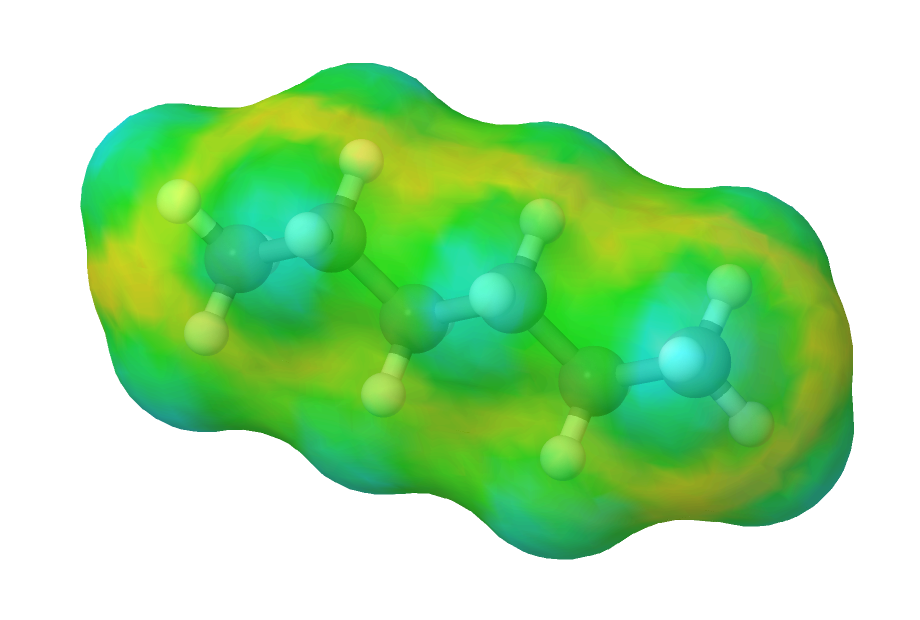
\includegraphics[width=0.45\textwidth]{img/n-hexane-cosmo.png}}
\subfloat[perfluorohexano]
{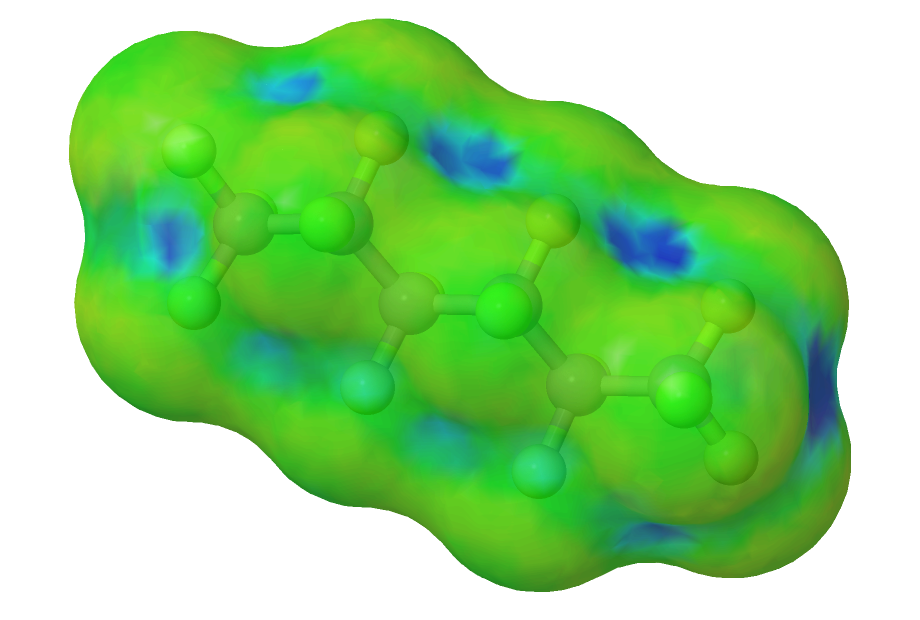
\includegraphics[width=0.45\textwidth]{img/perfluorohexane-cosmo.png}}
\caption{Superfície de contato para as moléculas de perfluorohexano e \emph{n}-hexano
obtidos utilizando o pacote COSab-GAMESS \cite{Gregerson2003} com o método BP86
e a função de base KTZVP, imagem renderizada pelo pacote JCOSMO
\cite{Gerber2010}.}
\label{fig:contact}
\end{figure}

Figuras simples
\begin{figure}[htb]	
\centering
{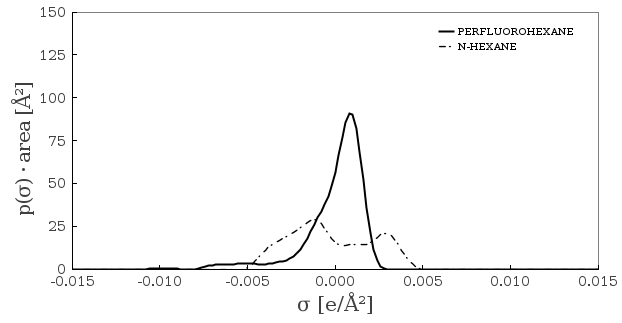
\includegraphics[width=0.8\textwidth]{img/COSMO-SAC.png}}
\caption{Perfil--$\sigma$ das moléculas de perfluorohexano e \emph{n}-hexano
obtidos utilizando o pacote COSab-GAMESS \cite{Gregerson2003} com o método BP86
e a função de base KTZVP.}
\label{fig:sigma_COSMO}
\end{figure}

 Figuras em arquivos.pdf
\begin{figure}[htb]
\centering
{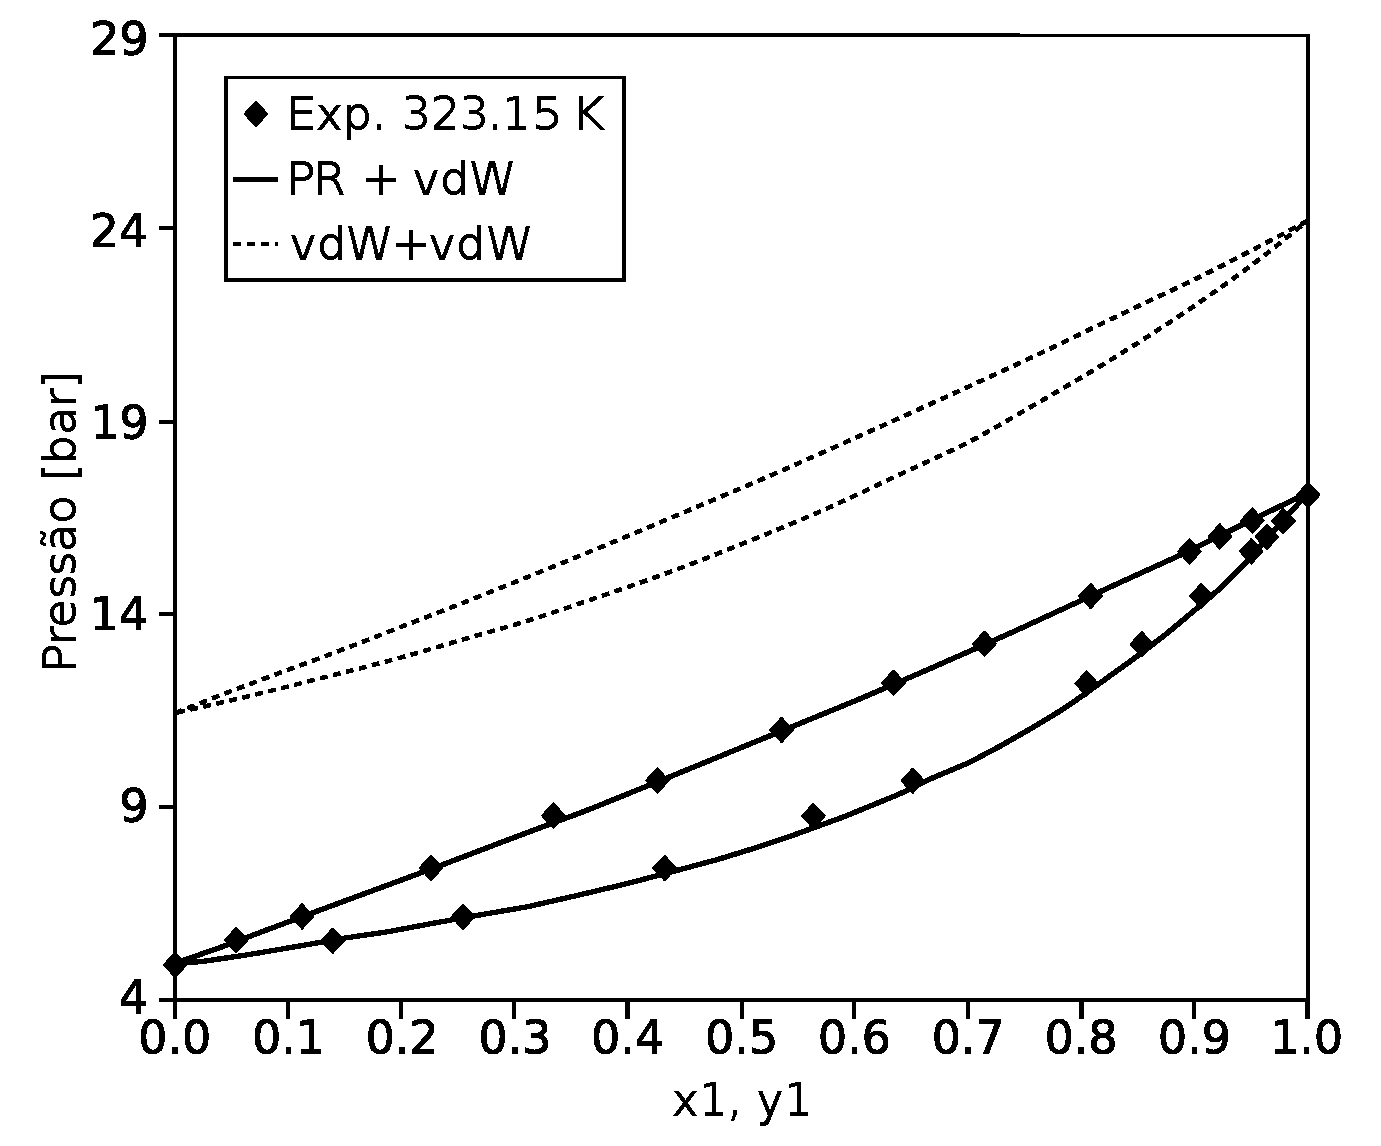
\includegraphics[width=0.6\textwidth]{img/propane_n-butane.pdf}}
\caption{Diagrama de equilíbrio $P-xy$ da mistura de de propano (1) e
\emph{n}-butano (2) calculados com as EoSs PR e vdW utilizando a regra de
mistura vdW}
\label{fig:eosvdwPropBut}
\end{figure}  


Fazer os gráficos, se necessário 
\begin{figure}[h]
\centering
\def\FunctionF(#1){-(#1)^4 + (#1)^3 +20}
\def\FunctionFd(#1){-4*(#1)^3 + 3*(#1)^2}
\def\FunctionFdd(#1){-12*(#1)^2 + 6*(#1)}
\subfloat[$f_2(x)$]
{\begin{tikzpicture}[scale=0.8]
\begin{axis}[
        axis y line=center,
        axis x line=middle, 
        axis on top=true,
        xmin=-1,
        xmax=1.5,
        ymin=19,
        ymax=21,
    ]
    \addplot [domain=-2:2.5, samples=100, 
    mark=none, ultra thick, blue]{\FunctionF(x)};
\node [right, blue] at (axis cs: 0.5,20.5) {$f_2(x)$};
\end{axis}
\end{tikzpicture}}
\subfloat[$\nabla f_2(x)$ e $\nabla^2 f_2(x)$]
{\begin{tikzpicture}[scale=0.8]
\begin{axis}[
        axis y line=center,
        axis x line=middle, 
        axis on top=true,
        xmin=-1,
        xmax=1,
        ymin=-1,
        ymax=2,
    ]
    \addplot [domain=-2:2.5, samples=100, 
    mark=none, ultra thick, orange]{\FunctionFd(x)};
    \addplot [domain=-2:2.5, samples=100, 
    mark=none, ultra thick, red]{\FunctionFdd(x)};
\node [right, orange] at (axis cs: 0.1,1.5) {$\nabla f_2(x)$};
\node [right, red] at (axis cs: 0.1,1.0) {$\nabla^2 f_2(x)$};
\end{axis}
\end{tikzpicture}}
\caption{$f_2 (x) = -x_1^4 + x_1^3 +20$.}
\label{fig:2f2}
\end{figure}
